\usepackage{beamer}
\documentclass{beamer}
\usepackage[utf8]{inputenc}
\usepackage{graphicx}
\usepackage{halloweenmath}
\usepackage{ulem}
\usepackage{cancel}

% https://www.overleaf.com/learn/latex/Beamer
\title{The Power of \LaTeX: \\ From Research Papers to R\'esum\'es}
\author{}

\begin{document}

\frame{\titlepage}

\begin{frame}{}
\begin{center}
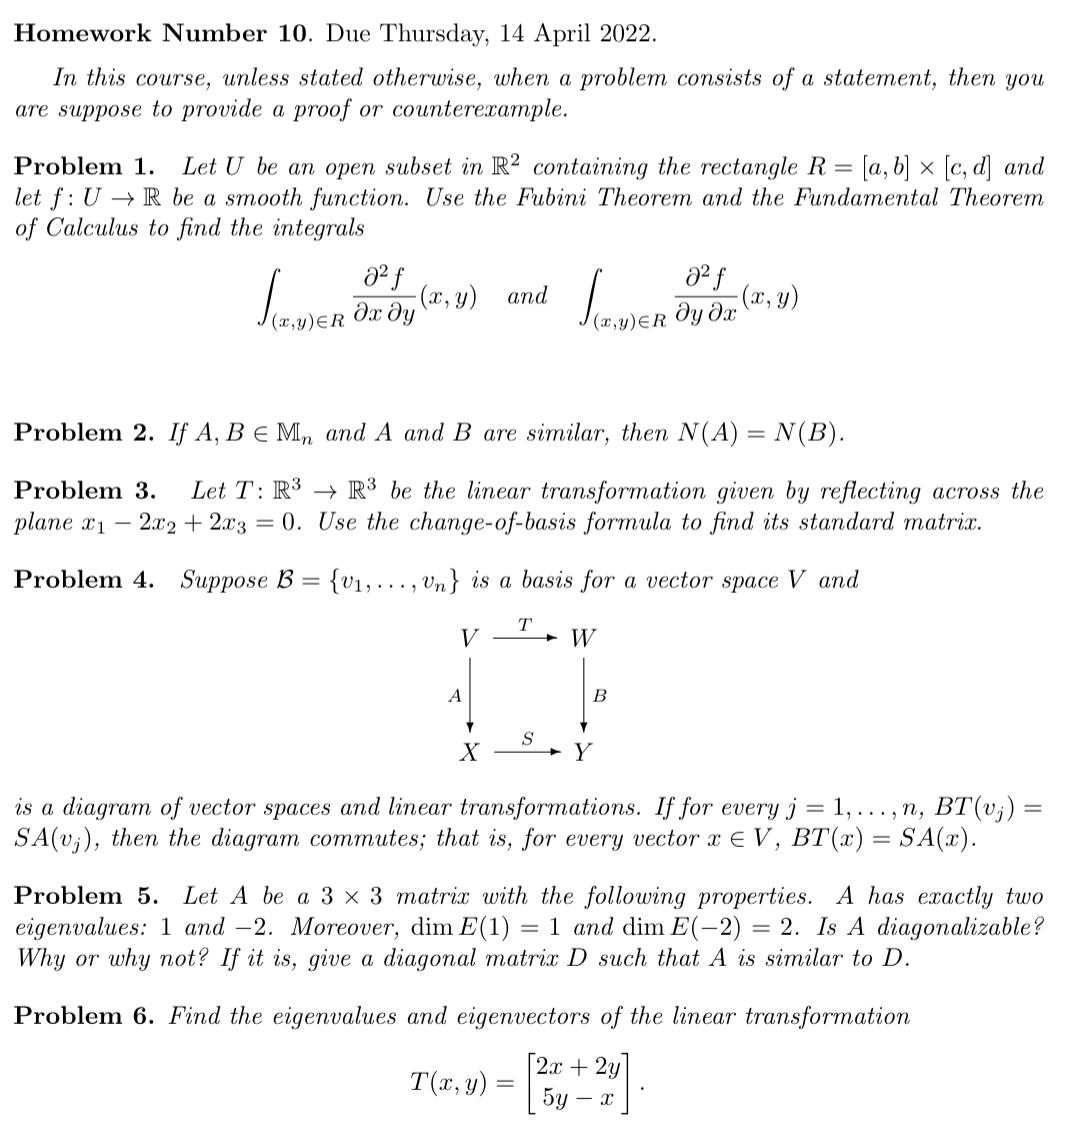
\includegraphics[scale=0.3]{blah.png}
\end{center}
\end{frame}

\begin{frame}{What is \LaTeX?}
\begin{itemize}
    \item A way of making documents with formatting, but in ``code'' instead of with an editor like Word or Google Docs
    \item Code is mixed in with plaintext to define formatting for that text
    \item Can be used to make all sorts of things!
    \begin{itemize}
        \item Documents with lots of formatting, like résumés or posters
        \item Papers with lots of symbols, like equations and proofs
        \item Presentations (like this one!)
    \end{itemize}
    \item There are tools to write it online, just like a Google Doc!
\end{itemize}
\end{frame}

\begin{frame}{}
\par\bigskip
  \vspace*{\fill}
  {\Large\bfseries Let's try it out!}\par\smallskip
  Go to overleaf.com to start editing.
  \vspace*{\fill}
\end{frame}

\begin{frame}{Adding Tables, Lists, Images etc.}
    \LaTeX{} supports all the formatting that you would expect from Word or Google Docs. To demonstrate this, let us work through a simple example of writing a recipe book! \newline
    
    We will learn how to make Fried \sout{Chicken} Squirrel.
\end{frame}

\begin{frame}{\LaTeX{} environments}
    \begin{itemize}
        \item Environments define special formatting within a block
        \item \texttt{\ttfamily \textbackslash begin\{environment\}} and \texttt{\ttfamily \textbackslash end\{environment\}}, and then text inside is formatted in a specific way
        \begin{itemize}
            \item The \textttt{itemize} environment styles \texttt{\ttfamily \textbackslash item} to make it look like a list item
            \item The \texttt{align} environment allows equations to be aligned
            \item The \texttt{tabular} environment styles its content as a table (and takes extra parameters for table styling)
        \end{itemize}
    \end{itemize}
\end{frame}

\begin{frame}{Equations}
    Let's say a professor gives you this equation, and you want to type it into your notes or a homework assignment:
    \begin{equation*}
    \nabla J_{\theta_j}(\theta)=\frac1m\sum_{i=1}^{m}(h_\theta(x^{(i)})-y^{(i)})x_{j}^{(i)}
    \end{equation*}
    How would you write this in Google Docs or Microsoft Word?
\end{frame}

\begin{frame}{Example: Calculus}
    Let's start with a basic calculus problem. 
    \begin{equation*}
    \int_{0}^{1} x^2 dx
    \end{equation*}
\end{frame}

\begin{frame}{Example: Proof}
    How would we write a proof---for example, a proof that the sum of two even numbers is even?
\end{frame}

\begin{frame}{Example: Normal Distribution}
    How would we write this equation?
    \begin{align*}
    f(x) = \frac{1}{\sigma \sqrt{2\pi} } e^{-\frac{1}{2}\left(\frac{x-\mu}{\sigma}\right)^2}
    \end{align*}
    How would you write this in Google Docs or Microsoft Word?
\end{frame}

\begin{frame}{So, when should I use \LaTeX?}
    \xcancel{at night}
    % 
\includegraphics[scale=0.2]{latex.jpg}
\end{frame}

\begin{frame}{So, when should I use \LaTeX?}
    \begin{itemize}
        \item There are tons of classes where \LaTeX{} can come in handy!
        \begin{itemize}
            \item Discrete Structures \& Algorithms
            \item Math (especially more proof and symbol-heavy courses)
            \item Machine Learning
            \item Labs in the sciences with equations
        \end{itemize}
        \item Résumés -- allows you to add information easily, without lots of reformatting work
        \item Research papers
    \end{itemize}
\end{frame}

\begin{frame}{Résumés}
\begin{center}
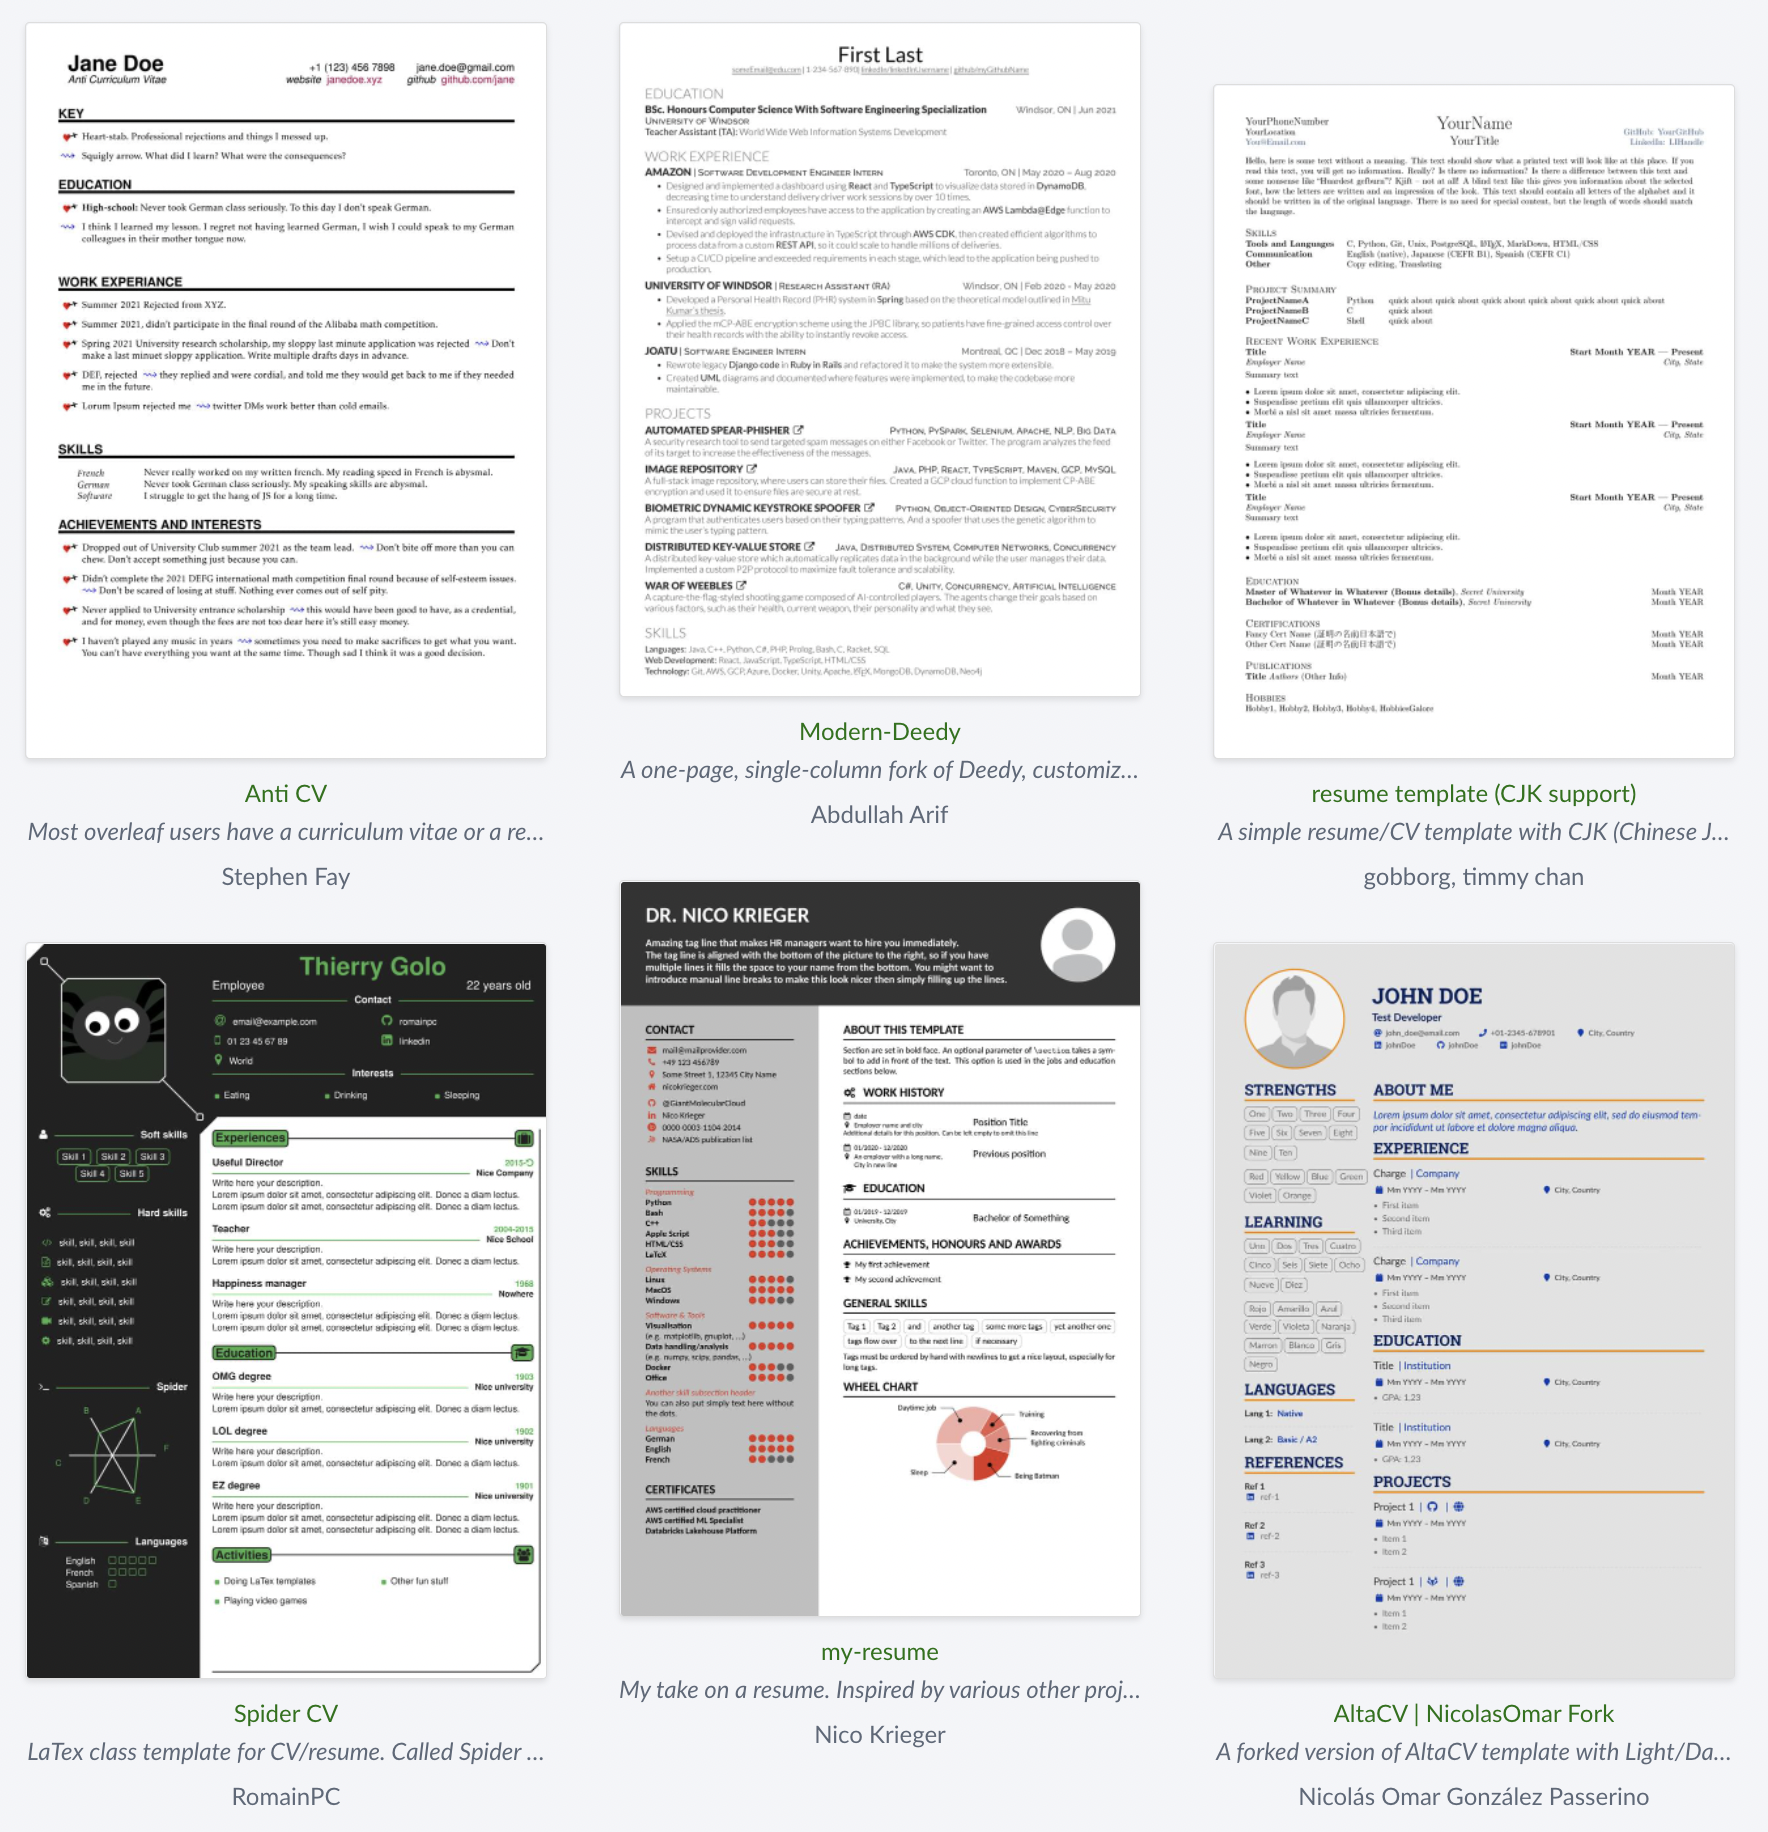
\includegraphics[scale=0.25]{resumes.png}
\end{center}
\end{frame}

\begin{frame}{Other Cool Things in \LaTeX}
    \begin{itemize}
        \item Macros -- custom commands with user-defined parameters that can expand into bigger commands
        \item Community packages, like \texttt{halloweenmath}! $\pumpkin \mathwitch \mathghost$
    \end{itemize}
\end{frame}

\begin{frame}{And when shouldn't I use \LaTeX?}
    \LaTeX{} is not the best tool for everything. For example, we didn't need \LaTeX{} to make this presentation\ldots and yet we did.
    \newline\newline
    In general, if you think \LaTeX{} is overkill for a project, it probably is.
    \newline\newline
    But the payoff is that you only need to focus on the content of your document---not endless typesetting details.
\end{frame}

\begin{frame}{}
\begin{center}
\par\bigskip
  {\Large\bfseries Thank you!}\par\smallskip
  \end{center}
\end{frame}


\end{document}
